\documentclass[12pt,addpoints]{exam}
\usepackage[utf8]{inputenc}
\usepackage{lastpage}
\usepackage{amsmath}
\usepackage{amsfonts}
\usepackage{amssymb}
\usepackage{enumerate}
\usepackage{mdframed}
\usepackage{array}
\usepackage{graphics}
\usepackage{graphicx}
\usepackage{listings}
\usepackage{skak}
\usepackage{tikz}
\usetikzlibrary{arrows}
\usepackage{tkz-berge}
\usepackage{algpseudocode}
\usepackage{hyperref}

% Paramètres globaux
\bonuspointpoints{point \emph{bonus}}{points \emph{boni}}
\parindent 0cm
\hqword{Question}
\hpword{Sur}
\hsword{Note}
\htword{Total}

% Réponses
%\printanswers

% En-tête et pieds de page
\headrule
\cfoot{\thepage /\pageref{LastPage}}
\lhead{CS Games --- Informatique théorique}
\rhead{Hiver 2016}
\newcommand{\headrulewidth}{0.4pt}
\newcommand{\footrulewidth}{0.4pt}

% Raccourcis
\newcommand{\bigo}{\mathcal{O}}
\newcommand{\N}{\mathbb{N}}
\newcommand{\R}{\mathbb{R}}

% Algorithmes
\algrenewcommand\algorithmicwhile{\textbf{tant que}}
\algrenewcommand\algorithmicfunction{\textbf{fonction}}
\algrenewcommand\algorithmicend{\textbf{fin}}
\algrenewcommand\algorithmicdo{\textbf{faire}}
\algrenewcommand\algorithmicfor{\textbf{pour}}
\algrenewcommand\algorithmicif{\textbf{si}}
\algrenewcommand\algorithmicelse{\textbf{sinon}}
\algrenewcommand\algorithmicthen{\textbf{alors}}
\algrenewcommand\algorithmicreturn{\textbf{retourner}}
\algrenewcommand\algorithmicrepeat{\textbf{faire}}
\algrenewcommand\algorithmicuntil{\textbf{tant que}}
\newcommand{\enteteproc}[2]{\vskip\baselineskip \hspace*{\fill} \algorithmicprocedure~\Call{#1}{#2} \hspace*{\fill} \vskip\baselineskip}
\newcommand{\entetefunc}[3]{\vskip\baselineskip \hspace*{\fill} \algorithmicfunction~\Call{#1}{#2} : #3 \hspace*{\fill} \vskip\baselineskip}

% Graphes
\tikzset{VertexStyle/.style={shape=circle, fill=black, inner sep=0pt, outer sep=0pt, minimum size=1.5mm, draw}}

\begin{document}
	
\allowdisplaybreaks

\thispagestyle{empty}
~\vfill
\ifprintanswers
  \vskip 1.2cm
  \centerline{\Large\textbf{Solution de l'épreuve}}
  \vskip 0.5cm
\else
  \vskip 1.2cm
  \centerline{\Large\textbf{Épreuve d'informatique théorique}}
  \vskip 1.2cm
\fi
\hrule \vskip \baselineskip
Cette épreuve contient 20 questions réparties en 4 thèmes de 5 questions chacun~:
\begin{enumerate}
  \item La combinatoire;
  \item La théorie des graphes;
  \item La théorie des jeux et des énigmes;
  \item Les probabilités.
\end{enumerate}
La pondération est la même pour chacune des questions. Bonne chance !
\vskip \baselineskip \hrule
\vfill~
\newpage

\begin{questions}

% Combinatoire
\uplevel{Les questions suivantes portent sur la \textbf{combinatoire}, c'est-à-dire la théorie qui consiste à compter ou énumérer des objets.}

% Compter des mots
\question
On dit d'une chaîne binaire $w$ qu'elle \emph{évite} un motif $u$ si elle ne s'écrit pas sous la forme $w = xuy$, où $x$ et $y$ sont des mots quelconques (possiblement vides).
\begin{parts}
  \part Pour tout entier $n \geq 0$, soit $A(n)$ le nombre de chaînes binaires de longueur $n$ qui évitent le motif $0$. Donnez la valeur de $A(n)$ pour tout $n$.
  \part De la même façon, soit $B(n)$ le nombre de chaînes binaires de longueur $n$ qui évitent le motif $00$. Donnez la valeur de $B(n)$ pour toute valeur de $n$.
  \part Même question, mais avec $C(n)$ le nombre de chaînes binaires qui évitent le motif $000$.
\end{parts}

% Arbres binaires
\question
Un \emph{arbre binaire} est une arborescence dont chaque sommet a au plus $2$ enfants. Pour tout entier $n \geq 0$, soit $A(n)$ le nombre d'arbres de $n$ noeuds.
\begin{parts}
  \part Montrez que les premières valeurs de $A(n)$ sont bien celles illustrées dans le tableau ci-bas~:
  \begin{center} \begin{tabular}{c|ccccc}
    $n$    & 0 & 1 & 2 & 3 & 4 \\
    \hline
    $A(n)$ & 1 & 1 & 2 & 5 & 14 \\
  \end{tabular} \end{center}
  \part Il est bien connu que $A(n)$ vérifie les équations suivantes~:
  \begin{eqnarray*}
    A(0) & = & 1, \\
    A(n) & = & \sum_{i=0}^{n-1} A(i)A(n-i-1).
  \end{eqnarray*}
  Justifiez ces deux équations. \emph{Indice~:} Réfléchissez à la construction récursive des arbres binaires.
\end{parts}

% Numéros de téléphone
\question
Combien existe-t-il de numéros de téléphone de $10$ chiffres (on suppose que les $10^{10}$ possibilités sont toutes valides) qui contiennent au moins une fois chacun des chiffres impairs ? Par exemple, le numéro $418$-$937$-$5351$ contient les chiffres $1$, $3$, $5$, $7$ et $9$, de sorte qu'il devrait être compté.
\begin{solution}
Il est plus facile de compter d'abord le nombre $n$ de numéros de téléphones pour lesquels il manque au moins un chiffre impair. Dénotons par $N_i$ l'ensemble des numéros de téléphone dans lesquels le chiffre $i$ n'apparaît pas. Alors clairement, 
$$n = \left| N_1 \cup N_3 \cup N_5 \cup N_7 \cup N_9 \right|.$$
Évidemment, les ensembles $N_1$, $N_3$, $N_5$, $N_7$ et $N_9$ ne sont pas disjoints et donc on doit utiliser le principe d'inclusion-exclusion. Tout d'abord, notons que $|N_i| = 9^{10}$ pour $i = 1,3,5,7,9$ puisqu'il suffit d'exclure, à chaque position, le chiffre interdit (on a donc $9$ choix à chaque position). En suivant cette logique, on remarque que $|N_i \cap N_j| = 8^{10}$ pour $i,j$ impairs et distincts, puis $|N_i \cap N_j \cap N_k| = 7^{10}$, $|N_i \cap N_j \cap N_k \cap N_\ell| = 6^{10}$ et finalement $|N_i \cap N_j \cap N_k \cap N_\ell \cap N_m| = 5^{10}$.

Il ne nous reste qu'à utiliser le principe d'inclusion-exclusion. On obtient
\begin{eqnarray*}
  n & = & \left| N_1 \cup N_3 \cup N_5 \cup N_7 \cup N_9 \right| \\
    & = & (|N_1| + |N_2| + |N_3| + |N_4| + |N_5|) \\
    &   & - (|N_1 \cap N_2| + |N_1 \cap N_3| + |N_1 \cap N_4| + \ldots + |N_4 \cap N_5|) \\
    &   & + (|N_1 \cap N_2 \cap N_3| + |N_1 \cap N_2 \cap N_4| + \ldots + |N_3 \cap N_4 \cap N_5|) \\
    &   & - (|N_1 \cap N_2 \cap N_3 \cap N_4| + |N_1 \cap N_2 \cap N_3 \cap N_5| + \ldots + |N_2 \cap N_3 \cap N_4 \cap N_5|) \\
    &   & + |N_1 \cap N_2 \cap N_3 \cap N_4 \cap N_5| \\
    & = & C(5,1) \cdot 9^{10} - C(5,2) \cdot 8^{10} + C(5,3) \cdot 7^{10} - C(5,4) \cdot 6^{10} + C(5,5) \cdot 5^{10} \\
    & = & 9228691000.
\end{eqnarray*}
Le nombre de numéros de téléphone cherché est donc
$$10^{10} - 9228691000 = 771309000.$$
\end{solution}

% Chemins dans une grille
\question
Considérez une grille de $r$ rangées et $c$ colonnes (voir Figure~\ref{F:grille}). Dans cette question, on s'intéresse à compter le nombre de chemins à partir du point $(0,0)$ jusqu'au point $(c,r)$ n'utilisant que des déplacements vers la droite (identifiés par la lettre $d$) et vers le haut (identifiés par $h$). Donnez une formule qui compte le nombre de chemins distincts de $(0,0)$ vers $(c,r)$, pour toutes valeurs $r,c \geq 1$.

% Nombres répétitifs
\question
On dit d'un nombre entier qu'il est \emph{répétitif} si tous ses chiffres en base $10$ sont identiques. Par exemple, $33$ et $999$ sont des nombres répétitifs. Aussi, soit $E$ un ensemble de $12$ nombres distincts quelconques entre $1$ et $99$ inclusivement. Montrez qu'il existe au moins deux nombres $x,y \in E$ tels que $x - y$ est un nombre répétitif.
\begin{solution}
Soit $X$ l'ensemble des nombres entre $1$ et $99$. Il y a au moins deux solutions à ce p
roblème.
\textbf{Solution 1}. Remarquons que si un nombre n'a qu'un seul chiffre, il est nécessairement répétitif. Par conséquent, il suffit de montrer qu'on a nécessairement deux nombres dans $E$ qui ont une différence d'au plus $9$. Pour $i = 0,1,\ldots,11$, soit $T_i = \{x \in X \mid 9i \leq x \leq 9i+9\}$ (autrement dit, les $T_i$ sont les tiroirs). Par le principe des tiroirs, si on choisit un ensemble $E$ de $12$ nombres entre $1$ et $99$, alors il existe $x, y \in E$ tels que $x \in T_i$, pour un certain entier $i$. Comme $9i \leq x,y \leq 9i + 9$, alors $|x - y| \leq (9i + 9) - 9i = 9$, c'est-à-dire que $x - y$ ou $y - x$ est un nombre répétitif.

\textbf{Solution 2}. On constate également que si $|x - y|$ est un multiple de $11$, alo rs $|x - y|$ est un nombre répétitif. Pour $i = 0,1,\ldots,10$, soit $T_i = \{x \in X \mid x \bmod 11 = i$ (autrement dit, on place les nombres dans le tiroir correspondant à l eur reste lorsqu'on les divise par $11$). Par le principe des tiroirs, il existe $x,y \in T_i$ pour un certain entier $i$, c'est-à-dire que $x \bmod 11 = y \bmod 11$. On en conclut que $(x - y) \bmod 11 = 0$, c'est-à-dire que $x - y$ ou $y - x$ est un multiple de $11$ entre $1$ et $99$, qui est un nombre répétitif.
\end{solution}

% Graphes
\uplevel{Les questions suivantes portent sur la \textbf{théorie des graphes}.
Un \emph{graphe simple} est un couple $G = (V,E)$ où $V$ est son ensemble de \emph{sommets} et $E \subseteq \mathcal{P}_2(V)$ est son ensemble d'\emph{arêtes}, où $\mathcal{P}_2(V)$ dénote l'ensemble des paires d'éléments distincts de $V$. Par exemple, le graphe $G = (V,E)$ défini par les ensembles
$$V = \{a,b,c,d\} \quad \text{et} \quad E = \{\{a,b\}, \{a,c\}, \{b,c\}, \{c,d\}\}$$
est représenté à la figure \ref{F:graphe}. À noter que dans un graphe simple, il n'y a pas d'arête multiple ni de boucle (une arête d'un sommet vers lui-même).}

% Familles de graphes
\question
Certaines familles de graphes simples sont souvent utilisées. En voici quelques-unes (voir figure~\ref{F:familles})~:
\begin{enumerate}[(i)]
  \item Pour tout entier $n \geq 1$, le graphe \emph{complet} de $n$ sommets $K_n$;
  \item Pour tout entier $n \geq 3$, le \emph{cycle} de $n$ sommets $C_n$;
  \item Pour tout entier $n \geq 3$, la \emph{roue} de $n + 1$ sommets $W_n$;
  \item Pour tout entier $n \geq 1$, l'\emph{hypercube} de dimension $n$ est noté $H_n$;
  \item Pour toute paire d'entiers $m,n \geq 1$, le graphe \emph{biparti complet} $K_{m,n}$;
\end{enumerate}
Pour toutes valeurs $n$ et $m$ bien définies, donnez le nombre d'arêtes des graphes suivants~:
\begin{parts}
  \part $K_n$;
  \part $C_n$;
  \part $W_n$;
  \part $H_n$;
  \part $K_{m,n}$.
\end{parts}

% Transversaux d'arêtes
\question
Soit $G = (V,E)$ un graphe simple. On dit d'un ensemble de sommets $U \subseteq V$ qu'il est un \emph{transversal d'arêtes} si chaque arête de $G$ a au moins une de ses extrémités dans $U$, c'est-à-dire que pour toute arête $\{u,v\} \in E$, on a $u \in U$ ou $v \in U$. Par exemple, dans le graphe de la figure \ref{F:graphe}, l'ensemble $\{a,c\}$ est un transversal d'arêtes. Un transversal d'arête $U$ est dit \emph{minimum} pour $G$ s'il n'existe aucun transversal d'arêtes $U'$ de plus petite cardinalité, c'est-à-dire tel que $|U'| < |U|$.

Pour toutes valeurs de $n$ et $m$ bien définies, donnez la taille d'un transversal d'arêtes minimum des graphes suivants~:
\begin{parts}
  \part $K_n$;
  \part $C_n$;
  \part $W_n$;
  \part $H_n$;
  \part $K_{m,n}$.
\end{parts}

% Problème HAMD
\question
On dit d'un graphe $G$ qu'il est \emph{hamiltonien} s'il admet au moins un cycle passant par chaque sommet \textbf{exactement} une fois.

Soit HAMD le problème de \emph{décider} si un graphe simple $G$ est hamiltonien ou non et soit HAM le problème de \emph{trouver} un cycle hamiltonien dans un graphe $G$ (on retourne la valeur \emph{rien} si un tel cycle n'existe pas). Autrement dit, on considère les deux fonctions suivantes~:
\begin{itemize}
  \item \Call{EstHamiltonien}{$G$ : graphe} : booléen;
  \item \Call{CycleHamiltonien}{$G$ : graphe} : cycle ou \emph{rien}.
\end{itemize}
Montrez que les deux problèmes sont de même difficulté à complexité polynomiale près. En d'autres termes, si $\textsc{EstHamiltonien}$ utilise un temps constant, alors on peut implémenter $\textsc{CycleHamiltonien}$ de telle sorte qu'elle utilise un temps polynomial (et vice-versa). \emph{Remarque~:} Vous devez écrire du pseudocode implémentant chacune des deux fonctions par rapport à l'autre.
\begin{solution}
Supposons d'abord que \textsc{CycleHamiltonien} utilise un temps constant. Alors la fonction
\begin{algorithmic}[1]
  \Function{EstHamiltonien}{$G$ : graphe} : booléen
    \State \Return \Call{CycleHamiltonien}{$G$}~$\neq$~rien
  \EndFunction
\end{algorithmic}
a également une complexité constante.

Réciproquement, supposons que \textsc{EstHamiltonien} utilise un temps constant et considérons la fonction suivante~:
\begin{algorithmic}[1]
  \Function{CycleHamiltonien}{$G = (V,E)$ : graphe} : cycle ou rien
    \If{$\neg \Call{EstHamiltonien}{G}$}
      \State \Return rien
    \Else
      \While{il existe $v \in V$ tel que $\deg(v) > 2$}
        \State Soit $v$ un sommet de degré au moins $3$
        \For{$u \in G.\Call{Voisins}{v}$}
          \State Soit $H$ le graphe obtenu de $G$ en supprimant $\{u,v\}$
          \If{$\Call{EstHamiltonien}{H}$}
            \State $G \leftarrow H$
          \EndIf
        \EndFor
      \EndWhile
      \State \Return l'unique cycle de $G$
    \EndIf
  \EndFunction
\end{algorithmic}
Sa complexité est de $\bigo(m(m + n)) = \bigo(m^2)$ qui est bien polynomiale.
\end{solution}

% Coloriages
\question\label{Q:kparti}
Étant donnés un graphe non orienté $G = (V,E)$ et un entier positif $k$, on dit d'une fonction $c : V \rightarrow \{1,2,\ldots,k\}$ qu'elle est un \emph{$k$-coloriage} de $G$ si pour toute arête $\{u,v\} \in E$, on a $c(u) \neq c(v)$, c'est-à-dire que deux sommets adjacents ont une couleur différente. Si $G$ peut être colorié à l'aide de $k$ couleurs, alors on dit qu'il est $k$-coloriable.

D'autre part, on dit que $G$ est $k$-parti s'il existe des ensembles $V_1, V_2, \ldots, V_k$ tels que
\begin{enumerate}
  \item $V_1 \cup V_2 \cup \cdots \cup V_k = V$,
  \item $V_i \cap V_j = \emptyset$ et
  \item Pour tout arête $\{u,v\}$, si $u \in V_i$ et $v \in V_j$, alors $i = j$.
\end{enumerate}
Autrement dit, on peut partitionner l'ensemble de sommets $V$ en $k$ morceaux de sorte que les arêtes reliant deux sommets dans un même morceau sont interdites.

Montrez que tout graphe $k$-parti est $k$-coloriable.

% P-équivalence coloriages
\question
Soit $k$-COLORD le problème de \emph{décider} si un graphe non orienté $G$ est $k$-coloriable et $k$-COLOR le problème de \emph{trouver} un $k$-coloriage de $G$. Montrez que les problèmes $k$-COLORD et $k$-COLOR sont de même difficulté à complexité polynomiale près. \emph{Indice~:} La question~\ref{Q:kparti} devrait vous être utile.

% Jeux
\uplevel{Les questions suivantes portent sur la \textbf{théorie des jeux et des énigmes}.}

% Jeu de Nim
\question
Cette question porte sur le célèbre \emph{jeu de Nim}, aussi appelé \emph{jeu des allumettes}. Il s'agit d'un jeu à deux joueurs, appelés joueur A et joueur B, qui, à tour de rôle, doivent retirer 2, 3 ou 4 allumettes d'un tas d'allumettes. Initialement, on suppose qu'il y a $n$ allumettes, où $n \geq 1$. Le gagnant est celui qui retire la ou les dernières allumettes.

On dit d'un joueur qu'il a une \emph{stratégie gagnante} s'il peut gagner à tous les coups, peu importe ce que l'autre joueur décide de faire.

Expliquez sous quelle condition le joueur A ou le joueur B a une stratégie gagnante au jeu de Nim. \emph{Remarque~:} Dans le jeu de Nim, lorsque la valeur de $n$ est fixée, un des deux joueurs a nécessairement une stratégie gagnante.

% Échecs
\question
(Tiré du livre \emph{The Chess Mysteries of the Arabian Knights}, de R. Smullyan) Considérez la position suivante aux échecs.
\fenboard{8/8/8/1r1b4/B7/8/8/3k4 w - - 0 20}
\[ \showboard \]
La position du roi blanc a été cachée. De plus, on ne sait pas si c'est au tour de blanc ou noir de jouer.

Devinez quelle est la position du roi blanc, sachant que tous les coups précédents ont été légaux et qu'il n'y a qu'une solution possible.
\begin{solution}
La solution se trouve à \href{https://www.chess.com/forum/view/fun-with-chess/where-is-the-king-retrograde-analysis}{https://www.chess.com/forum/view/fun-with-chess/where-is-the-king-retrograde-analysis}.
\end{solution}

% Jeu d'échecs à deux coups
\question
Nous nous intéressons maintenant à une variante du jeu d'échecs traditionnels, dans laquelle chaque joueur peut jouer \emph{deux coups consécutifs}. Sachant que ce sont les blancs qui commencent et les noirs qui jouent en deuxième, montrez qu'avec cette variante, les noirs ne peuvent pas avoir une stratégie gagnante. \emph{Indice~:} procédez par l'absurde.

% Jet d'oeuf
\question
Vous vous trouvez dans un édifice de $100$ étages (numérotées de $1$ à $100$) avec $2$ oeufs. Chacun de ces oeufs a la particularité qu'il existe un nombre $n$ entre $1$ et $100$ (le nombre $n$ est le même pour les $2$ oeufs) tel que~:
\begin{itemize}
  \item si vous le laissez tomber d'un étage entre $1$ et $n$, alors il ne se casse pas;
  \item si vous le laissez tomber d'un étage entre $n + 1$ et $100$, alors il se casse.
\end{itemize}
Proposez une stratégie optimale pour deviner la valeur de $n$ qui minimise le nombre de fois que vous devez laisser tomber un oeuf. Justifiez votre réponse.

% Tonneaux de vin
\question
Vous êtes un homme riche et sans scrupule, ayant en votre possession un nombre illimité d'esclaves. Dans six heures aura lieu un banquet auquel sont conviés de nombreux invités. Cependant, vous venez d'apprendre que, parmi les $128$ tonneaux de vin que vous avez l'intention de servir, exactement un d'entre eux a été empoisonné. De plus, vous savez que les effets du poison, lorsque ingéré, ne se manifestent qu'après quatre heures. Vous décidez donc de tester les tonneaux de vins sur vos esclaves.

Proposez une stratégie qui vous permettra de déterminer avec certitude quel tonneau de vin est empoisonné, en minimisant le nombre d'esclaves sacrifiés. Plus bas sera le nombre, plus de points vous obtiendrez.

% Probabilités
\uplevel{Les questions suivantes portent sur la \textbf{théorie des probabilités}.}

% Générateur non-uniforme
\question
Considérez une fonction $\Call{NonUniforme}$ qui retourne au hasard la valeur $0$ avec probabilité $0.7$ et la valeur $1$ avec probabilité $0.3$. On suppose que c'est la seule fonction que vous pouvez utiliser pour simuler le hasard, les autres fonctions habituelles n'étant pas disponibles. Évidemment, vous pouvez appeler la fonction $\Call{NonUniforme}$ autant de fois que vous le désirez. En utilisant la fonction $\Call{NonUniforme}$, donnez le pseudocode d'une fonction $\Call{Uniforme}$ qui retourne la valeur $0$ ou $1$ avec probabilité uniforme.
\begin{solution}
\end{solution}

% Algorithmes et probabilités
\question
Supposez que pour un problème de décision donné $P$, vous ayez à votre disposition deux algorithmes, appelés $A$ et $B$. Vous avez également les informations suivantes~:
\begin{itemize}
  \item Lorsque l'algorithme $A$ retourne \emph{vrai}, vous savez que la réponse au problème $P$ est nécessairement \emph{vrai}. En revanche, si l'algorithme $A$ retourne \emph{faux}, il peut se tromper avec probabilité $0.05$.
  \item Lorsque l'algorithme $B$ retourne \emph{faux}, vous savez que la réponse au problème $P$ est nécessairement \emph{faux}. En revanche, si l'algorithme $B$ retourne \emph{vrai}, il peut se tromper avec probabilité $0.1$.
\end{itemize}
Est-il possible de construire un algorithme $C$ à partir des algorithmes $A$ et $B$ de telle sorte que l'algorithme $C$ retourne \emph{vrai} ou \emph{faux} sans jamais se tromper ? Justifiez.

% Arbre binaire de recherche
\question
Considérez un arbre binaire de recherche quelconque. On suppose que les services suivants sont disponibles pour tout arbre $T$~:
\begin{itemize}
  \item $T.\Call{estVide}$ retourne vrai si et seulement si $T$ est un arbre vide;
  \item $T.\Call{contenu}$ retourne la valeur contenue dans la racine de l'arbre $T$;
  \item $T.\Call{taille}$ retourne le nombre total de noeuds dans l'arbre $T$;
  \item $T.\Call{gauche}$ retourne le sous-arbre gauche de $T$ (possiblement vide);
  \item $T.\Call{droit}$ retourne le sous-arbre droit de $T$ (possiblement vide).
\end{itemize}
En n'utilisant que les services ci-haut, donnez le pseudocode d'une fonction
\begin{center}
\Call{ValeurAleatoire}{$T$ : arbre binaire de recherche}
\end{center}
qui retourne au hasard une valeur présente dans l'arbre $T$ (on suppose qu'une valeur ne peut pas apparaître plus d'une fois, pour simplifier). Notez que chaque valeur doit avoir la \textbf{même probabilité} d'être retournée. Aussi, vous pouvez supposer qu'il existe une fonction \Call{random}{$n$} qui retourne un nombre entier entre $0$ et $n - 1$ (inclusivement) au hasard avec probabilité uniforme.

% Échantillon
\question
Considérez un ensemble de $n$ entiers quelconques (distincts). On souhaite former un échantillon de $i$ entiers distincts ($1 \leq i \leq n$) tirés aléatoirement parmi les $n$ entiers disponibles (c'est donc un tirage sans remise). Pour cela, on utilise l'algorithme suivant~:
\begin{algorithmic}[1]
  \Function{Échantillon}{$E$ : ensemble d'entiers, $i$ : entier}
    \State $S \gets \emptyset$
    \While{$S.\Call{taille}{} \neq i$}
      \State $e \gets $ un élément choisi aléatoirement dans $E$
      \If{$e \notin S$}
        \State $S.\Call{insérer}{e}$
      \EndIf
    \EndWhile
    \State \Return $S$
  \EndFunction
\end{algorithmic}
\begin{parts}
  \part Quelle est la probabilité que l'algorithme ne termine pas ?
  \part Montrez qu'en moyenne, le nombre de tours de boucle \textbf{tant que} effectués est $\bigo(n\log n)$, où $n$ est la taille de l'ensemble $E$ et $0 \leq i \leq n$.
\end{parts}

% Échantillon
\question
Considérez un tableau $T$ de $n$ entiers non ordonnés et pas nécessairement distincts. Soit $x$ un entier apparaissant $k$ fois dans le tableau $T$. Clairement, $0 \leq k \leq n$.

On s'intéresse aux nombres de valeurs inspectées lorsqu'on effectue une fouille linéaire du tableau $T$. Plus précisément, on considère l'algorithme suivant ($T$ est indicé à partir de $0$)~:
\begin{algorithmic}[1]
  \Function{EstDansTableau}{$T$ : tableau, $x$ : élément}
    \State Soit $n$ le nombre d'éléments dans $T$
    \State $i \gets 0$
    \While{$i < n$ \textbf{et} $T[i] \neq x$}
      \State $i \gets i + 1$
    \EndWhile
    \State \Return $i < n$
  \EndFunction
\end{algorithmic}
Pour toutes valeurs de $k$ possibles, donnez une formule indiquant le nombre de valeurs moyennes qu'on s'attend à inspecter? Vous devez donner une expression \textbf{exacte}, c'est-à-dire pas avec la notation $\bigo$. \emph{Indice~:} Considérez séparément les cas $k = 0$, $k = 1$ et $k > 1$.

\end{questions}

\begin{figure}
  \centering
  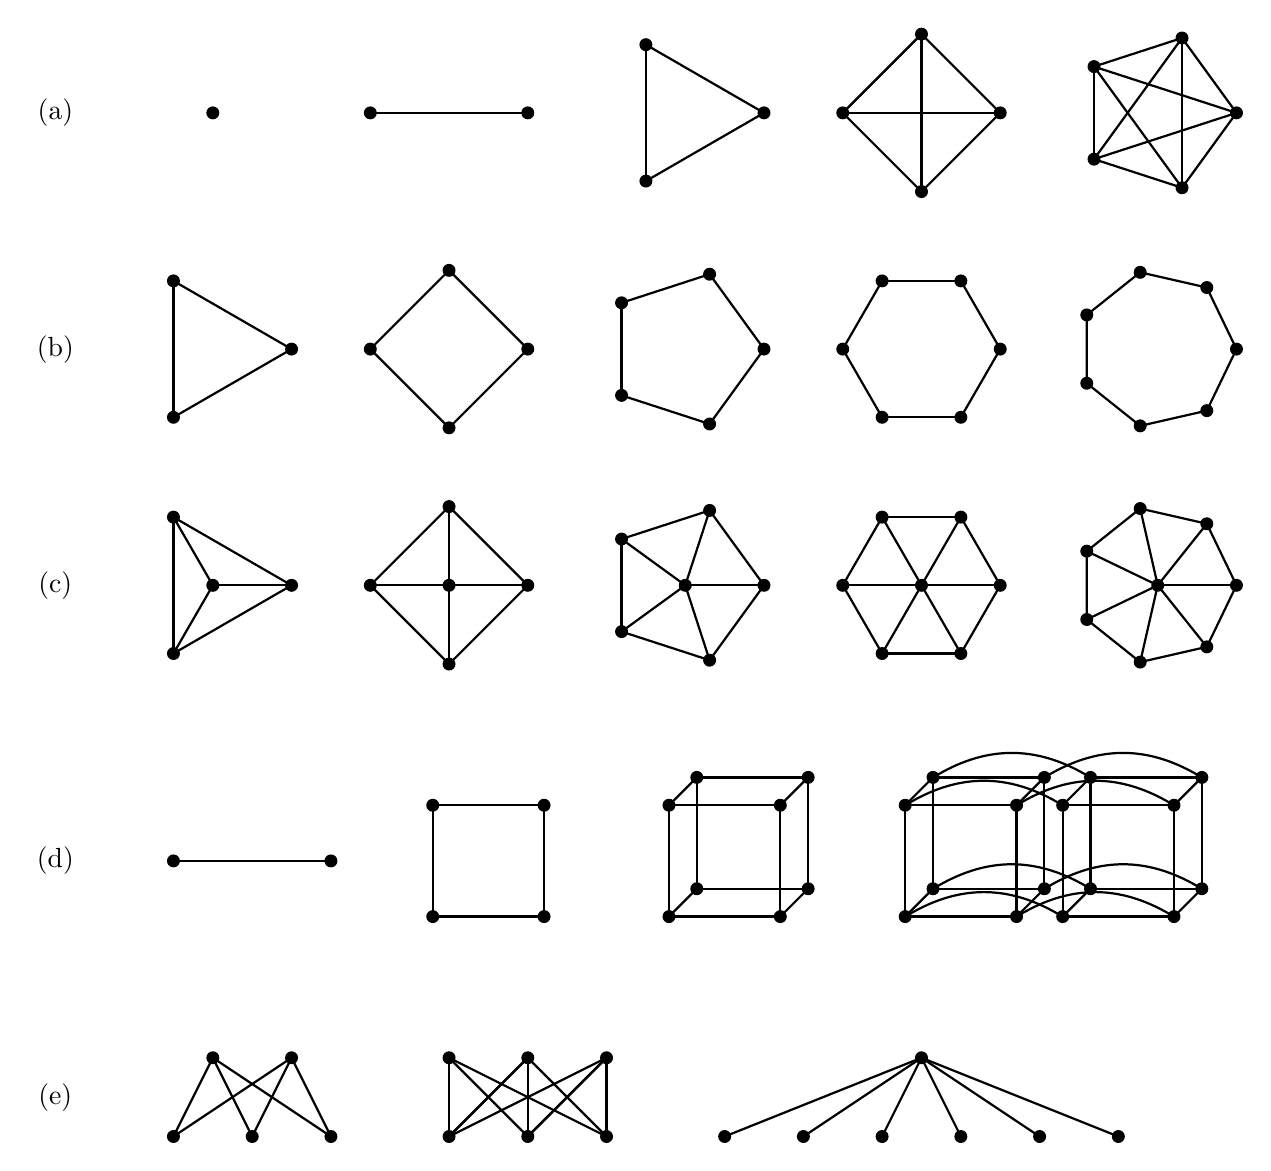
\begin{tikzpicture}
    % Complets
    \begin{scope}[xshift=-1cm, yshift=0cm]
      \node at (0,0) {(a)};
    \end{scope}
    \begin{scope}[xshift=0cm, yshift=0cm]
      \SetVertexNoLabel \Vertices{circle}{A}
    \end{scope}
    \begin{scope}[xshift=4cm, yshift=0cm]
      \SetVertexNoLabel \Vertices{circle}{A,B}
      \Edges(A,B)
    \end{scope}
    \begin{scope}[xshift=7cm, yshift=0cm]
      \SetVertexNoLabel \Vertices{circle}{A,B,C}
      \Edges(A,B,C,A)
    \end{scope}
    \begin{scope}[xshift=10cm, yshift=0cm]
      \SetVertexNoLabel \Vertices{circle}{A,B,C,D}
      \Edges(A,B,C,D,A,C,B,D)
    \end{scope}
    \begin{scope}[xshift=13cm, yshift=0cm]
      \SetVertexNoLabel \Vertices{circle}{A,B,C,D,E}
      \Edges(A,B,C,D,E,A,C,E,B,D,A)
    \end{scope}
    % Cycles
    \begin{scope}[xshift=-1cm, yshift=-3cm]
      \node at (0,0) {(b)};
    \end{scope}
    \begin{scope}[xshift=1cm, yshift=-3cm]
      \SetVertexNoLabel \Vertices{circle}{A,B,C}
      \Edges(A,B,C,A)
    \end{scope}
    \begin{scope}[xshift=4cm, yshift=-3cm]
      \SetVertexNoLabel \Vertices{circle}{A,B,C,D}
      \Edges(A,B,C,D,A)
    \end{scope}
    \begin{scope}[xshift=7cm, yshift=-3cm]
      \SetVertexNoLabel \Vertices{circle}{A,B,C,D,E}
      \Edges(A,B,C,D,E,A)
    \end{scope}
    \begin{scope}[xshift=10cm, yshift=-3cm]
      \SetVertexNoLabel \Vertices{circle}{A,B,C,D,E,F}
      \Edges(A,B,C,D,E,F,A)
    \end{scope}
    \begin{scope}[xshift=13cm, yshift=-3cm]
      \SetVertexNoLabel \Vertices{circle}{A,B,C,D,E,F,G}
      \Edges(A,B,C,D,E,F,G,A)
    \end{scope}
    % Roues
    \begin{scope}[xshift=-1cm, yshift=-6cm]
      \node at (0,0) {(c)};
    \end{scope}
    \begin{scope}[xshift=1cm, yshift=-6cm]
      \SetVertexNoLabel \Vertices{circle}{A,B,C}
      \Edges(A,B,C,A)
      \Vertex{O}
      \Edge(O)(A)
      \Edge(O)(B)
      \Edge(O)(C)
    \end{scope}
    \begin{scope}[xshift=4cm, yshift=-6cm]
      \SetVertexNoLabel \Vertices{circle}{A,B,C,D}
      \Edges(A,B,C,D,A)
      \Vertex{O}
      \Edge(O)(A)
      \Edge(O)(B)
      \Edge(O)(C)
      \Edge(O)(D)
    \end{scope}
    \begin{scope}[xshift=7cm, yshift=-6cm]
      \SetVertexNoLabel \Vertices{circle}{A,B,C,D,E}
      \Edges(A,B,C,D,E,A)
      \Vertex{O}
      \Edge(O)(A)
      \Edge(O)(B)
      \Edge(O)(C)
      \Edge(O)(D)
      \Edge(O)(E)
    \end{scope}
    \begin{scope}[xshift=10cm, yshift=-6cm]
      \SetVertexNoLabel \Vertices{circle}{A,B,C,D,E,F}
      \Edges(A,B,C,D,E,F,A)
      \Vertex{O}
      \Edge(O)(A)
      \Edge(O)(B)
      \Edge(O)(C)
      \Edge(O)(D)
      \Edge(O)(E)
      \Edge(O)(F)
    \end{scope}
    \begin{scope}[xshift=13cm, yshift=-6cm]
      \SetVertexNoLabel \Vertices{circle}{A,B,C,D,E,F,G}
      \Edges(A,B,C,D,E,F,G,A)
      \Vertex{O}
      \Edge(O)(A)
      \Edge(O)(B)
      \Edge(O)(C)
      \Edge(O)(D)
      \Edge(O)(E)
      \Edge(O)(F)
      \Edge(O)(G)
    \end{scope}
    % Hypercubes
    \begin{scope}[xshift=-1cm, yshift=-9.5cm]
      \node at (0,0) {(d)};
    \end{scope}
    \begin{scope}[xshift=1.5cm, yshift=-9.5cm]
      \SetVertexNoLabel \Vertices{circle}{A,B}
      \Edges(A,B)
    \end{scope}
    \begin{scope}[xshift=4.5cm, yshift=-9.5cm, rotate=45]
      \SetVertexNoLabel \Vertices{circle}{A,B,C,D}
      \Edges(A,B,C,D,A)
    \end{scope}
    \begin{scope}[xshift=7.5cm, yshift=-9.5cm]
      \SetVertexNoLabel
      \begin{scope}[rotate=45]
      \Vertices{circle}{A,B,C,D}
      \begin{scope}[xshift=5mm] \Vertices{circle}{E,F,G,H} \end{scope}
      \end{scope}
      \Edges(A,B,C,D,A)
      \Edges(E,F,G,H,E)
      \Edge(A)(E)
      \Edge(B)(F)
      \Edge(C)(G)
      \Edge(D)(H)
    \end{scope}
    \begin{scope}[xshift=10.5cm, yshift=-9.5cm]
      \SetVertexNoLabel
      \begin{scope}[rotate=45]
      \Vertices{circle}{A,B,C,D}
      \begin{scope}[xshift=5mm] \Vertices{circle}{E,F,G,H} \end{scope}
      \end{scope}
      \Edges(A,B,C,D,A)
      \Edges(E,F,G,H,E)
      \Edge(A)(E)
      \Edge(B)(F)
      \Edge(C)(G)
      \Edge(D)(H)
      \begin{scope}[xshift=2cm]
      \begin{scope}[rotate=45]
      \Vertices{circle}{Ap,Bp,Cp,Dp}
      \begin{scope}[xshift=5mm] \Vertices{circle}{Ep,Fp,Gp,Hp} \end{scope}
      \end{scope}
      \Edges(Ap,Bp,Cp,Dp,Ap)
      \Edges(Ep,Fp,Gp,Hp,Ep)
      \Edge(Ap)(Ep)
      \Edge(Bp)(Fp)
      \Edge(Cp)(Gp)
      \Edge(Dp)(Hp)
      \Edge[style={bend left}](A)(Ap)
      \Edge[style={bend left}](B)(Bp)
      \Edge[style={bend left}](C)(Cp)
      \Edge[style={bend left}](D)(Dp)
      \Edge[style={bend left}](E)(Ep)
      \Edge[style={bend left}](F)(Fp)
      \Edge[style={bend left}](G)(Gp)
      \Edge[style={bend left}](H)(Hp)
      \end{scope}
    \end{scope}
    % Bipartis complets
    \begin{scope}[xshift=-1cm, yshift=-12cm]
      \node at (0,-0.5) {(e)};
    \end{scope}
    \begin{scope}[xshift=1cm, yshift=-12cm]
      \SetVertexNoLabel
      \Vertices[x=0,y=0]{line}{A,B}
      \Vertices[x=-0.5,y=-1]{line}{C,D,E}
      \Edges(A,C,B,D,A,E,B)
    \end{scope}
    \begin{scope}[xshift=4cm, yshift=-12cm]
      \SetVertexNoLabel
      \Vertices[x=0,y=0]{line}{A,B,C}
      \Vertices[x=0,y=-1]{line}{D,E,F}
      \Edges(A,D,B,E,C,F,B,D,C,E,A,F)
    \end{scope}
    \begin{scope}[xshift=7.5cm, yshift=-12cm]
      \SetVertexNoLabel
      \Vertices[x=2.5,y=0]{line}{A}
      \Vertices[x=0,y=-1]{line}{B,C,D,E,F,G}
      \Edge(A)(B)
      \Edge(A)(C)
      \Edge(A)(D)
      \Edge(A)(E)
      \Edge(A)(F)
      \Edge(A)(G)
    \end{scope}
  \end{tikzpicture}
  \caption{Quelques familles de graphes célèbres. (a) Le graphe complet $K_n$ pour $n = 1,2,3,4,5$. (b) Le cycle $C_n$ pour $n = 3,4,5,6,7$. (c) La roue $W_n$ pour $n = 3,4,5,6,7$. (d) L'hypercube $H_n$ pour $n = 1,2,3,4$. (e) Les graphes bipartis $K_{2,3}$, $K_{3,3}$ et $K_{1,6}$.}\label{F:familles}
\end{figure}

\begin{figure}
  \centering
  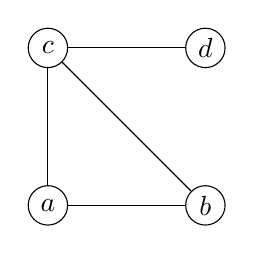
\begin{tikzpicture}[sommet/.style={draw, circle, inner sep=0pt, minimum size=5mm}]
    % Sommets
    \node[sommet] at (0,0) (a) {$a$};
    \node[sommet] at (2,0) (b) {$b$};
    \node[sommet] at (0,2) (c) {$c$};
    \node[sommet] at (2,2) (d) {$d$};
    % Arêtes
    \path (a) edge (b) edge (c);
    \path (c) edge (b) edge (d);
  \end{tikzpicture}
  \caption{Le graphe $G = (V,E)$, où $V = \{a,b,c,d\}$ et $E = \{\{a,b\}, \{a,c\}, \{b,c\}, \{c,d\}\}$.}\label{F:graphe}
\end{figure}

\begin{figure}
  \centering
  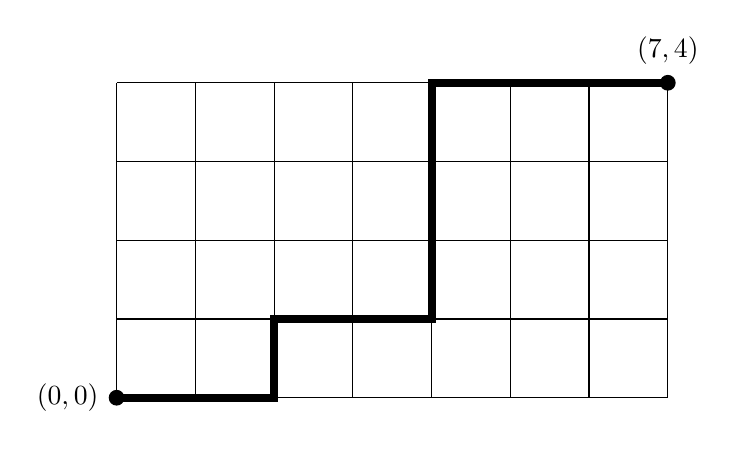
\begin{tikzpicture}[sommet/.style={fill=black, circle, inner sep=0pt, minimum size=2mm}]
    % Grille
    \draw (0,0) grid (7,4);
    % Sommets
    \node[sommet, label=180:{$(0,0)$}] at (0,0) (d) {};
    \node[sommet, label=90:{$(7,4)$}]  at (7,4) (f) {};
    % Chemin
    \draw[line width=1mm] (0,0) -- ++ (1,0) -- ++ (1,0) -- ++ (0,1) -- ++ (1,0) -- ++ (1,0) -- ++ (0,1) -- ++ (0,1) -- ++ (0,1) -- ++ (1,0) -- ++ (1,0) -- ++ (1,0);
  \end{tikzpicture}
  \caption{Une grille avec $r = 4$ et $c = 7$. Le chemin $ddhddhhhddd$ est représenté par un trait gras.}\label{F:grille}
\end{figure}

\end{document}
